\chapter{Own Work}
\label{ch:ownwork}
\section{Stable Diffusion Pipeline}

One of the thesis's main goals was to build a diffusion-based pipeline to enhance synthetic tracking data like from the Synthehicle dataset \autoref{ch:synthehicle} and evaluate them afterward. This section will focus on the software engineering side behind the pipeline implementation, explaining core features and functionality.

\subsection{Programming language and project structure}

For the programming language, Python was chosen as it has great libraries for image parsing (\href{https://github.com/python-pillow/Pillow}{"Pillow"}) and the \href{https://github.com/huggingface/diffusers}{"diffusers" package}, which allows fast integration of various hugging face models, especially in the Stable Diffusion space. Also, one of the core modules, ALDM \cite{li2024aldm}, is also mostly written in Python, which makes integrating this project into the pipeline much easier.

Python allows the split of the project into multiple packages \autoref{fig:package_diagram_sd_pipeline}, which later could be distributed easily via \href{https://conda-forge.org/}{Conda-Forge} or \href{https://pypi.org/}{PyPi}. Therefore, the pipeline is structured in a highly modular way, ensuring easy extendability while keeping installation requirements minimal. Each module is currently maintained within a mono repository, managed by \href{https://github.com/pdm-project/pdm}{"PDM"} which is installed on top of a  \href{https://docs.anaconda.com/miniconda/}{"Conda"} environment. This unconventional package management approach offers three main advantages:

First, Conda enables the installation of packages from Conda Forge and binaries, which is particularly beneficial for optimized, platform-specific package builds.

Second, PDM assists in managing dependencies through its lock file and mono repository support.

Third, this unconventional approach allows for the installation of packages before the PDM install, facilitating the resolution of package dependencies such as \href{https://github.com/pytorch/pytorch}{PyTorch} to compile instructions from YoloX.

\begin{figure}[H]
  \centering
  \includegraphics[width=\textwidth]{figures/own_work/pipeline/package_diagram.pdf}
  \caption{Package Diagram for the implemented modules}
  \label{fig:package_diagram_sd_pipeline}
  \clearpage
\end{figure}

\subsection{Dataflow and Stream Structure}

Each function that is encapsulated in different pipeline methods accesses the pipeline's data stream. The data stream contains the image that should be processed, metadata, and other information, like bounding boxes or depth information. The implementation of the stream allows three data types: 
    
\begin{figure}[H]
\begin{lstlisting}[language=Python]
      stream:   Dict[str, str | PIL.Image] |
                Tuple[Dict[str, str | PIL.Image]] | 
                None
\end{lstlisting}
\caption{Stream Data Type (The type should be \textit{PIL.Image.Image}, but due to its length, it will be abbreviated to \textit{PIL.Image} throughout the rest of this thesis.}
\end{figure}

The dictionary is the fundamental structure that contains all the important information for an image. In this context, the "Tuple" datatype was chosen as the container for managing multiple images or inputs in one stream. Tuples were selected over lists to highlight the importance of order within the stream and to emphasize the functional concept of immutable variables.


\subsection{Functionality}
\label{subch:functionality}

The \textbf{Pipeline} class is the heart piece of the application and contains all functions for building and executing different image processing pipelines \autoref{fig:class_diagram_sd_pipeline}. The implementation mostly follows the builder pattern \cite{10.5555/186897} by building the pipeline with different methods and getting the result after executing the run method. Therefore, a pipeline is represented through class methods that are chained together, with each method describing a step in the pipeline. Each of them returns the class object itself with a modified state by adding a function to its function array. All functions are executed in the end by the \textit{run} method. 

The \textbf{SubPipeline} class is a wrapper class around the "private" constructor of the Pipeline class (Python does not allow private constructors and does not have any equivalent to C++ friend classes. The underlying implementation, therefore, does not forbid access to the constructor from outside of the Pipeline class) and returns an empty Pipeline. This class should be used to initialize SubPipelines for different Pipeline methods.

\begin{figure}[H]
  \centering
  \includegraphics[width=\textwidth]{figures/own_work/pipeline/class_diagram_sd-pipeline_components.pdf}
  \caption{Class Diagram for the pipeline component (functions with the self attribute are class methods, otherwise they are static methods)}
  \label{fig:class_diagram_sd_pipeline}
  \clearpage
\end{figure}


To provide a large amount of functionality, the pipeline offers different methods to manipulate the stream of data that is pushed from function to function.

\begin{itemize}
    \item \textit{init()}: The init method is the only static function of the pipeline class and allows the initialization of an empty Pipeline. It helps with the injection of a pipeline config that is injected into each module \ref{sec:modules},

    \item \textit{loop()}: The loop method allows the execution of its SubPipeline for a defined amount of time. The output of the SubPipeline is the input for the next iteration.

    \item \textit{collect()}: The collect method also allows the execution of its SubPipeline within a defined amount of time. Here, each iteration gets the same input, and the results are returned in a tuple of tuples or dictionaries.

    \item \textit{for\_each()}: The for\_each method is often combined with the step method if specific modules can only have one image dictionary as its input. The method allows the execution of a given SubPipeline for each element in a Tuple.

    \item \textit{parallel()}: The parallel method runs multiple pipelines parallel with the same input and stores its output in a tuple (the functions inside the function array are still called sequentially - the reason for that is the Graphic card storage that would be a bottleneck for most computers).

    \item \textit{split()}: The split method splits its input stream into different output streams, each going into a separate SubPipeline. The ratio can be defined in absolute numbers or percentages.

    \item \textit{flatten()}: The flatten method flattens the output streams by unpacking tuples for positive depth parameters. For negative depth parameters, it's the other way around; the input is wrapped in tuples.

    \item \textit{run()}: The run method is the final step of building a pipeline. This method iterates over the statement array and calls the different functions added by all methods before.

    \item \textit{\_inject\_image\_data()}: This method manipulates the image stream by inserting new image data into it. Mostly, it is only used by other functions to copy a stream into a SubPipeline.

\end{itemize}

The last two functions that are not explained in this section, \textit{step()} and \textit{prepare()}, will be part of the next section, which focuses on exploring the module architecture.

\section{Modules}
\label{sec:modules}

Modules contain the main logic of the Pipeline and support one specific feature. Every module's structure is defined by the module superclass, which is part of the "sd-pipeline-typing" package, also displayed in \autoref{fig:package_diagram_sd_pipeline}. Modules are differentiated into base modules, all modules implemented inside the sd-pipeline package, and package modules, where each package contains a different module. The base modules contain relevant IO features or easy formatting features, while the package modules contain larger features like complicated mapping tasks or difficult-based transformations.
\begin{figure}[H]
  \centering
  \includegraphics[width=\textwidth]{figures/own_work/pipeline/class_diagram_modules.pdf}
  \caption{Class Diagram describing the module architecture}
  \label{fig:class_diagram_module}
  \clearpage
\end{figure}

The module's interface is defined by two methods: the constructor, which initializes the module with the configuration object during pipeline programming, and the run method, which manipulates the data stream. This interface is established through the abstract class Module in the "sd-pipeline-typing" module. Additionally, the interface for configuration classes is provided within this package. All interfaces are implemented through inheritance, illustrated in \autoref{fig:class_diagram_module}.
Some modules also contain a static method named format\_stream for data stream manipulation, i.e. to assign segmentation or depth information to the appropriate images.

To integrate a module into the sd-pipeline, the \textit{prepare()} and \textit{step()} methods can be used. While the \textit{prepare()} method takes a callable as its only argument, allowing the format\_stream() method to gain access to the data stream, the \textit{step()} method takes a module as its parameter, adding the run method to the functions array and injecting the pipeline configuration. 

\subsection{Base Modules: pipeline-specific modules}

Some of the modules are directly implemented into the pipeline package. These modules contain core features and build the pipeline's data flow manipulation foundation. 
\\

The first and second ones are the I/O modules \textit{Load\_from\_fs} and \textit{Store\_to\_fs}. They are responsible for loading images into the Pipeline via the library "Pillow" and storing them afterward.
\\

The third I/O module \textit{Load\_bboxes\_from\_fs} loads bounding boxes from a JSON file into the pipeline stream, therefore providing metadata for the images that have to be matched with the help of other modules.
\\

\textit{Rename} and \textit{Resize} are two modules to manipulate an image by changing its name via a lambda function and resizing images with the help of the "Pillow" library. 
\\

The last four modules \textit{Group}, \textit{Multiply}, \textit{Sort}, and \textit{Filter} focus on manipulating not the images of the stream directly but changing the stream's behavior. \textit{Sort} sorts the dictionaries inside a stream by a given key, \textit{multiply} multiplies each dictionary by a defined number and \textit{group} groups $n$ streams together by combining all dictionaries from the same positions into a new tuple and filter removes image dictionaries that fail a predicate function.
\\

\subsection{Package Modules}

The package modules can be installed separately, and they are the main processing units of the pipeline. Therefore, this thesis will explain each of these modules in detail, also providing examples for the generated images and comparisons with a focus on object detection in \autoref{ch:evaluation}.
\subsubsection{CARLA}

\begin{figure}[H]
  \centering
  \includegraphics[clip, trim=0cm 3cm 0cm 0cm,width=\textwidth]{figures/own_work/modules/class_diagram_carla_module.pdf}
  \caption{Class Diagram describing the Carla script import architecture. The Carla module package is here presented as a black box. For more detail on how modules are structured, refer to \autoref{fig:class_diagram_module}}
  \label{fig:class_diagram_module_carla}
  \clearpage
\end{figure}

The CARLA module is logically the first module and facilitates data extraction from the CARLA Simulator (see \autoref{ch:carla}). Using the \href{https://pypi.org/project/carla/}{CARLA Python package}, it is possible to configure CARLA's simulation and export data such as semantic segmentation, depth information, and bounding boxes. To provide the pipeline user with complete flexibility for configuration, the module allows the loading of custom scripts called "Carla Scripts." These scripts are used to program the simulation. The interface "CarlaScriptInterface" is provided to help the user maintain the necessary structure (see \autoref{fig:class_diagram_module_carla}).

The module provides the functions \textit{pre()} and \textit{post()}, which are called before and after the \textit{run\_script()} function to set up the basic environment and clean up. The \textit{run\_script()} method itself is called from the carla\_module during the pipeline run, executing the script. 

Safety is a crucial topic, and it is important to acknowledge that this module should not be used in a public environment. The "Carla Scripts" are loaded without validation, which could allow malicious code to be executed during a pipeline run.

\subsubsection{ALDM}

ALDM (see \autoref{ch:aldm}) is the first step of the image generation process, allowing a segmentation map to be transformed into a realistic, detailed image with the help of a Stable Diffusion algorithm and a control net. To integrate the code into the pipeline, it had first been made installable as a package. Therefore, rewriting the original ALDM code and creating a wrapper around it to be called from my pipeline was necessary. Additionally, the configuration settings are extracted into a configuration class to make them accessible at the pipeline programming level.

\subsubsection{Image2Image}

The Image2Image module extends the ALDM processing by enabling further image manipulation after its initial creation. As described in \autoref{ch:controlnet}, image-to-image processes take an existing image as their base and generate a new one from it. This generation can be guided by ControlNets. This module implements multiple variations, including image-to-image without a ControlNet, the ControlNet trained on semantic segmentation by Lvmin Zhang \cite{zhang2023addingconditionalcontroltexttoimage}, the ControlNet trained on depth by Lvmin Zhang \cite{zhang2023addingconditionalcontroltexttoimage}, and a combination of both. All modules work with Stable Diffusion 1.5 \cite{rombach2022highresolution} as it was the only available Stable Diffusion checkpoint with a ControlNet trained on both inputs.

\subsubsection{Convert Seg Format \& Convert Depth Format}
To provide correctly formatted segmentation and depth information for the ControlNets in the image2image module, the segmentation maps and depth maps must be properly modified.
The convert-seg-format module offers methods to transform a semantic segmentation map from the Cityscapes dataset \cite{cordts2016cityscapesdatasetsemanticurban} format to the ade20k dataset \cite{zhou2019semantic} format and vice versa. This is essential because Sythehicle \cite{Herzog_2023_WACV} provides and ALDM \cite{li2024aldm} consumes Cityscape-formatted segmentation maps, while the ControlNet requires ADE-formatted segmentation maps.
The convert-depth-format module provides two functionalities. The first one inverts the depth map (Sythehicle provides depth information with the nearest objects being the darkest, while the depth control net requires the reverse), and the second one includes a denormalizer that allows a function to run on each pixel of a depth map, reverting possible normalizations.

\subsubsection{Upscale-Downscale-Details-Enhancer}

The upscale downscale module tries to enrich image data with more details by first up-scaling the image with the help of a latent diffusion network \cite{rombach2022highresolution} and then down-scaling it with "Pillow". This should help with missing details and broken proportions by adding/repairing them during the upscale process and not losing them completely during the downscale. In combination with the loop method provided by the pipeline, which can be found in \autoref{subch:functionality}, this module could enhance the image multiple times before passing it to the next pipeline method. Its idea originates from the DLSS-Algorithm developed by NVIDIA \cite{watson2020deeplearningtechniquessuperresolution} for PC-Games, which also takes a low-resolution image, upscales, and afterward downscales it to the monitor resolution to provide better image quality.

\subsubsection{Convert to COCO}

As the package name already states, this module converts an input stream into the COCO format \cite{lin2015microsoftcococommonobjects}, exporting the label files as JSON. With the help of the \textit{split()} method, \autoref{subch:functionality}, and some prepossessing functions, the input stream can be split to allow the dataset to contain the train, test, and validation labels. The purpose of this module is primarily to help with the evaluation through the \textit{yolox} module.

\subsubsection{YoloX}
The YoloX module is the main evaluator module providing object detection on COCO datasets \cite{lin2015microsoftcococommonobjects}. YoloX provides different models with different layer sizes, offering  large flexibility for training. The module wraps the \href{https://github.com/Megvii-BaseDetection/YOLOX}{YoloX package} \cite{yolox2021}, allowing it to be integrated into pipelines seamlessly.

\subsubsection{Finetuning}
A key feature of YoloX is the ease with which the model can be trained or fine-tuned. The pipeline is designed to facilitate the fine-tuning of existing checkpoints using newly generated data, ensuring that the model can be enhanced by that.

\subsubsection{Resulting checkpoints and evaluation}
After every epoch, YoloX provides a new checkpoint with the updated weights and training results consisting of the precision and recall values for each class. The module also exports them, providing the possibility to compare different pipeline configurations and use the trained checkpoint for other projects \autoref{ch:evaluation}.

\section{Visual and Object detection testing}
Another part of this thesis is the evaluation of the different modules and a detailed comparison between the results of different pipelines. Multiple tests regarding object detection have been run to test the performance and quality of the different results, and the output has been analyzed visually.

\subsection{Test setup}

For the major generation modules, small tests have been conducted to determine the best configurations. Following this, a dataset containing 300 segmentation maps was generated from six different settings within the Synthicle dataset (Town01-N-..., C01 - CO6, 50 segmentation maps from the selected scene) (\autoref{ch:synthehicle}) and the MUAD dataset (300 images out of the validation set, because annotations for the test set was not available) (\autoref{ch:muad}). Four main themes, daytime, dawn, rain, and night were applied to the  300 segmentation maps, resulting in 1,200 images. This process was repeated twice, ultimately producing 2 datasets, each containing a total of 2,400 finalized images.

Due to time constraints (the generation for every dataset took over 3 days), the images from other datasets were used as a base for new ones. For example, when using the image2image module, the output from the ALDM Module was taken as the new input instead of regenerating the images resulting from the ALDM modules. While this could carry graphical errors through the tests, new generations could also introduce new graphical errors, making this an efficient trade-off between time and dataset size.

The dataset generation and the later conducted tests run on two machines, with the first one having two NVIDIA Titans and the other one having an NVIDIA RTX 4070. On both machines, the tests were run with the same YoloX settings.

\subsubsection{Object detection with pre-trained model}

With the resulting images, object detection for the train images was conducted to measure the quality of the different data sets by looking at the average precision (AP) and average recall (AR) the pre-trained COCO weights for the YoloX model can achieve (more details on these measurements in \autoref{sec:test_results_object_detection}). 

\subsubsection{Object detection model finetuning}

With the resulting datasets, the YoloX reconfigured COCO weights were further fine-tuned and evaluated with 600 random images from the Cityscapes dataset to test if the module could be further optimized through data generated with a Stable Diffusion algorithm. As mentioned in \autoref{ch:cityscapes} the dataset was enhanced by adding foggy and rainy scenes to make detecting cars harder.

\section{Consistency and tracking testing}
Maintaining spatial and temporal consistency between different image generations is a problem most diffusion modules have. Four different test approaches were conducted to visualize the problem and test how spatial and temporal consistency could be preserved. For each test, the same six starting images were used.

\subsection{Test setup Baseline}
The Synthhicle dataset was used for these tests, as the images originate from videos and are, therefore, sequential. Per scene, 100 images were taken, and we are building the baseline for the other tests that will modify these images.

\subsection{Test setup ALDM}

This test focuses on generating 100 images with ALDM. The input was 100 segmentation maps that followed one another, resulting in a 10-second-long video with 10 frames per second.


\subsection{Test setup image to image, segmentation ControlNet}

\begin{figure}[H]
  \centering
  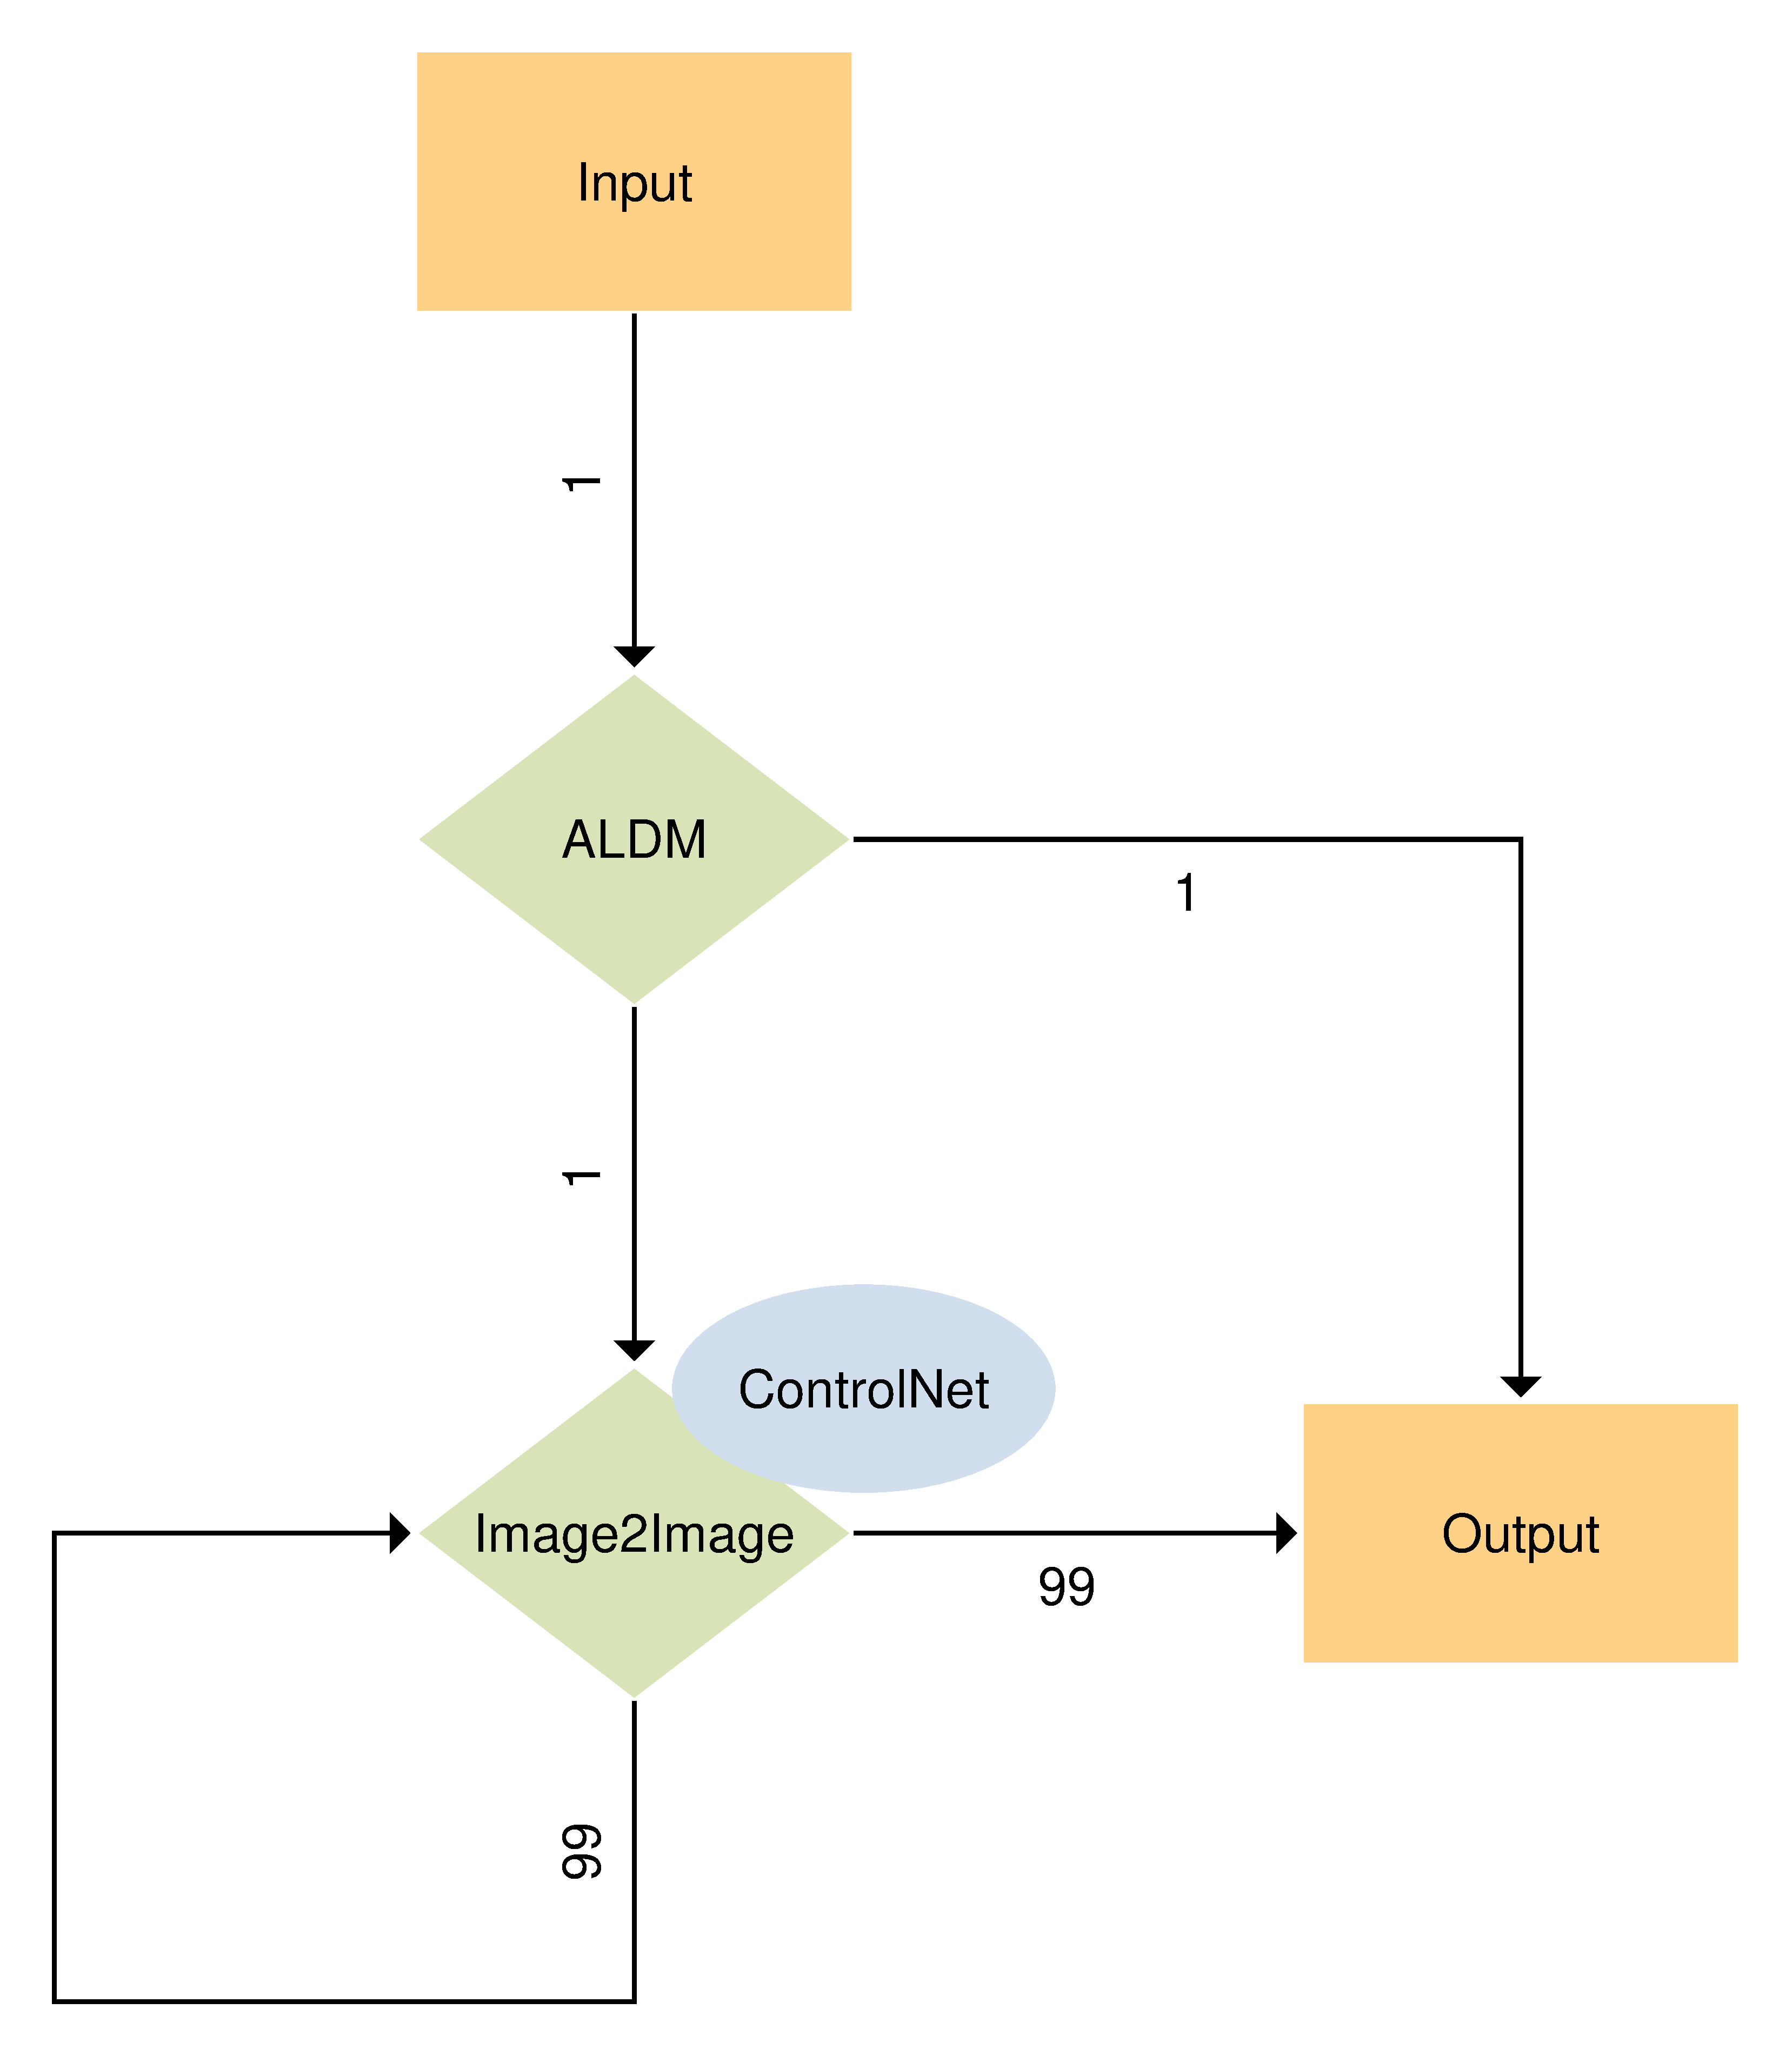
\includegraphics[width=0.5\textwidth]{figures/own_work/temporal_spacial_consistency/temporal_consistency_i2i_pipeline.pdf}
  \caption{Visitation of the i2i consistency pipeline}
  \label{fig:temporal_consistency_i2i_pipeline}
  \clearpage
\end{figure}

For the next test, as shown in \autoref{fig:temporal_consistency_i2i_pipeline}, only the first segmentation map is used as input for the ALDM module. The resulting image is the starting point for the image-to-image process, with every step generating a new frame with the previous output as its next input. To guide the generation for the following frame, the segmentation ControlNet is used together with the next fame segmentation map. The resulting video is 10 seconds long with 10 frames per second. During different tests, the prompt of the image-to-image module was changed to cover multiple scenarios. For the final result, the seed and the strength parameter were kept the same (see \autoref{sec:high_score_for_the_strength_parameter} and \autoref{sec:color_shifting_of_the_scenes} for more details).

\subsection{Test setup image-to-image, segmentation \& depth ControlNet}

This test has a similar test setup as the previous one, only differing in the used ControlNets, combining segmentation maps with depth information. 

\subsection{Image constancy evaluation}

To evaluate the consistency of these different videos, the previous image is compared to the current image via the Root Mean Square Error (RMSE; for calculation details, refer to the \href{https://github.com/up42/image-similarity-measures/blob/master/image_similarity_measures/quality_metrics.py}{used implementation}) to see how big the change between two consecutive frames is. This is compared to the synthetic image video (the baseline).


\subsection{Object tracking evaluation}

With the help of \href{https://github.com/ultralytics}{Ultralytics}, Bytetrack \cite{zhang2022bytetrackmultiobjecttrackingassociating}, and pertained Yolo v8 \cite{reis2024realtimeflyingobjectdetection} weights, every vehicle in the video was tracked during the 10 seconds and labeled with a unique ID. The IDs are assigned in ascending order, increasing by $1$ for each subsequent vehicle. If the tracking algorithm loses the car, a new ID is assigned. In the end, the difference between the number of IDs counted on the synthetic image video (the baseline) and the number of IDs is used as a metric for the quality of the generated cars and their stability between different frames.